\scanpage{16}
\mspage{8}
Ceci noté, on aura donc, si $j,j'\in J=\operatorname{Ob}\Pi_1$
\[
\begin{aligned}
\operatorname{Isom}_{\Pi_{1,\unsure{\mathrm f|\phi}}}(j,j')&\overset{\mathrm{dfn}}{=}\operatorname{Isom}(\widetilde{\mathfrak X}'[j],\widetilde{\mathfrak X}'[j'])\\
&\simeq\operatorname{Isom}_{\pi_1\text{-tors à droite}}(\widetilde{\mathfrak X}'(j),\widetilde{\mathfrak X}'(j'))
\end{aligned}
\]
la composition des chemins étant la composition des hom de $\pi_1$-tors\unsure{.} à droite.
\deleted{\unsure{Comme}} On a donc reconstruit 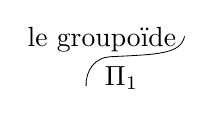
\begin{tikzpicture}[baseline=(object.base)]
\node[inner sep=0pt] (object) at (0,0) {$\Pi_1$};
\node[anchor=south,inner sep=0pt] at (-.25,.32) {\inserted{le groupoïde}};
\draw[line width=.3pt] (-.45,-.10) .. controls (-.46,.10) and (-.33,.26) .. (-.15,.27) .. controls (.45,.30) and (.75,.30) .. (.80,.53);
\end{tikzpicture} à l'aide de $\widetilde{\mathfrak X}'(J)$ et de l'opération libre (à droite) de $\pi_1$ sur $\widetilde{\mathfrak X}'(J)$.
\deleted{[les opérations} Comment reconstituer l'opération de $\mathcal G'$ sur $\Pi_1$ ? L'opération sur $\operatorname{Ob}\Pi_1=J$ n'est autre que l'opération donnée de $\mathcal G'$ sur $J$ (factorisant celle de $\unsure{\mathcal E'|\Sigma'}$). Soit $g\in\mathcal G'$, explicitons
\diagram{\begin{tikzcd}[ampersand replacement=\&]
\operatorname{Isom}_{\Pi_1}(j,j') \arrow[r,"{\substack{g_{\Pi_1}\\[-.3ex]\sim}}"] \arrow[d,equal] \& \operatorname{Isom}(gj,gj') \arrow[d,equal]\\
\operatorname{Isom}_{\pi_1}(\widetilde{\mathfrak X}'(j),\widetilde{\mathfrak X}'(j')) \arrow[r,"{\substack{?\\[-.3ex]\sim}}"] \& \operatorname{Isom}_{\pi_1}(\widetilde{\mathfrak X}'(gj),\widetilde{\mathfrak X}'(gj'))
\end{tikzcd}}
Pour ceci, considérons le 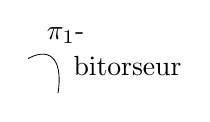
\begin{tikzpicture}[baseline=(word.base)]
\node[anchor=base west,inner sep=0pt] (word) at (0,0) {bitorseur};
\node[anchor=base east,inner sep=0pt] at (.15,.46) {\inserted{$\pi_1$-}};
\draw[line width=.3pt] (-.57,.22) .. controls (-.25,.39) and (-.13,.15) .. (-.19,-.22);
\end{tikzpicture}
\[
B_g\unsure{:}\subset\unsure{\mathcal E'|\Sigma'}\qquad\text{image inv. de }g\text{ par }\unsure{\mathcal E'|\Sigma'}\unsure{\mathbin{-}|\longrightarrow}\mathcal G'
\]
On note que l'on a (grâce à l'op. de $\unsure{\mathcal E'|\Sigma'}$ sur $\widetilde{\mathfrak X}'(I)$]
\[
\begin{aligned}
\widetilde{\mathfrak X}'(gj)&\simeq\widetilde{\mathfrak X}'(j)\mathbin{\wedge}_{\pi_1}B_g\\
\widetilde{\mathfrak X}'(gj')&\simeq\widetilde{\mathfrak X}'(j')\mathbin{\wedge}_{\pi_1}B_g
\end{aligned}
\]
\mspage{15}
